\documentclass[tikz]{standalone}
\usetikzlibrary{arrows}
\usetikzlibrary{arrows.meta}

\begin{document}
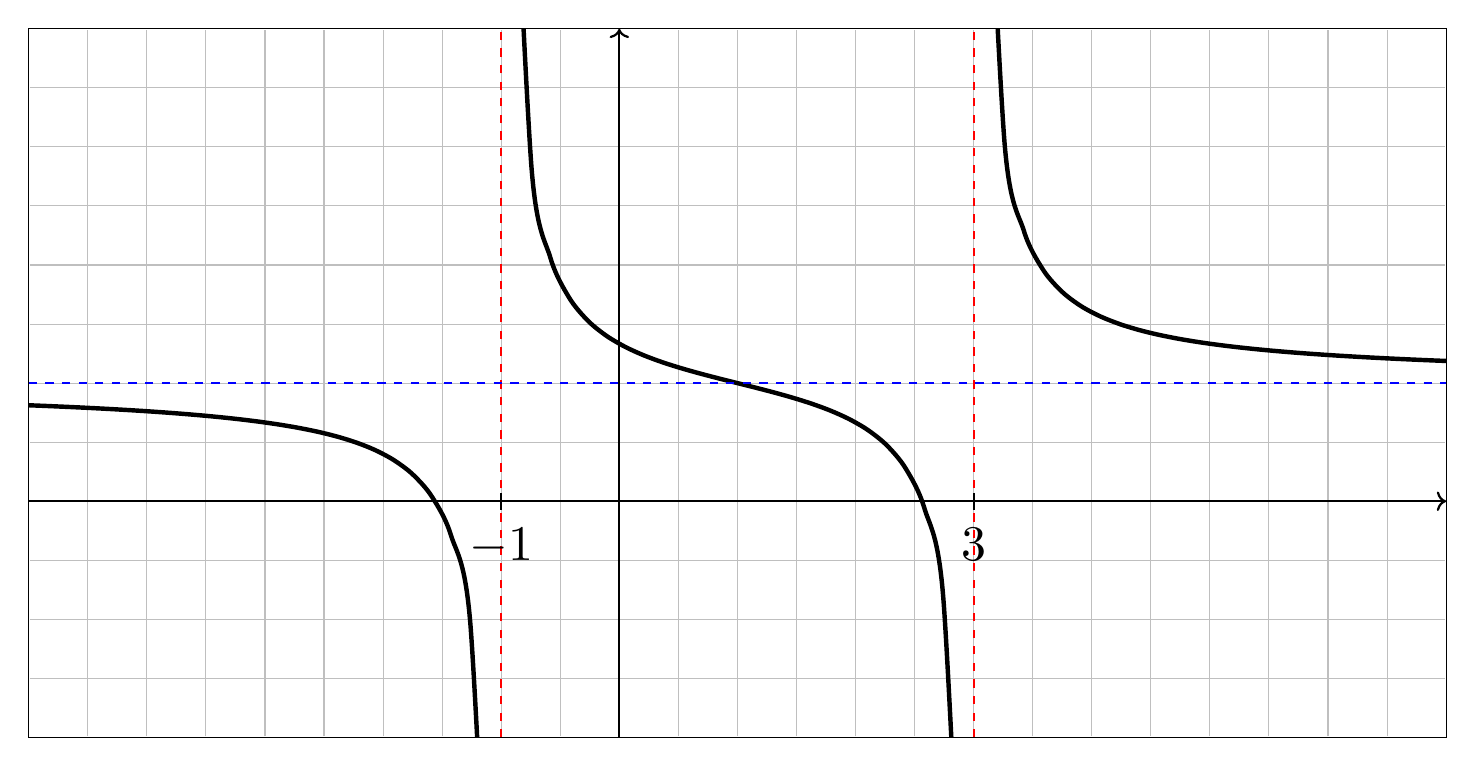
\begin{tikzpicture}[baseline=70,ultra thick,smooth,domain=-4:4,variable=\x,scale=1.5]

% create a white background with a black frame
\draw [thin,fill=white] (-5,-2) rectangle (7,4);  

% draw grid
\draw[xstep=0.5cm, ystep=0.5cm, lightgray, thin] (-4.99,-1.99) grid (6.99,3.99); 

% draw axes
\draw [->,thick] (-5,0) -- (7,0);
\draw [->,thick] (0,-2) -- (0,4);


\clip (-5,-2) rectangle (7,4);

% x / (x^2-4) + 1
\draw plot [domain=-5:-1.1] (\x,{1 + (\x-1) / ((\x-1)*(\x-1) - 4)}); 
\draw plot [domain=-0.9:2.9] (\x,{1 + (\x-1) / ((\x-1)*(\x-1) - 4)}); 
\draw plot [domain=3.1:7] (\x,{1 + (\x-1) / ((\x-1)*(\x-1) - 4)}); 

% asymptotes
\draw[dashed,red,thick] (-1,-2) -- (-1,4);
\draw[dashed,red,thick] (3,-2) -- (3,4);
\draw[dashed,blue,thick] (-5,1) -- (7,1);

% tick marks
\foreach \x in {-1,3} 
	\draw [thick] (\x cm,2pt) -- (\x cm,-2pt) node[below, scale=1.8] {$\x$};

\end{tikzpicture}
\end{document}
